\documentclass[tikz, crop, border=5pt]{standalone}

\usepackage{xcolor}
\usepackage{mathtools}

\DeclareMathOperator{\uniform}{\mathcal{U}}

\usetikzlibrary{
    positioning,
    arrows.meta
}

\tikzset{%
    random variable/.style={%
        circle,
        draw,
        inner sep = 0pt,
        outer sep = 0pt,
        minimum width=1cm
    },
    state/.style={%
        circle,
        draw,
        inner sep = 0pt,
        outer sep = 0pt,
        minimum width=1cm,
        fill=black!20
    },
    observed rv/.style={%
        random variable,
        fill=blue!20,
    },
    unobserved rv/.style={%
        random variable,
        fill=white,
    },
    arrow/.style={%
        >={Stealth[round]},
    },
    formula/.style={%
        rectangle,
        draw=gray,
        rounded corners=2pt,
        inner sep = 2pt,
        outer sep = 0pt,
        minimum width=12cm,
        minimum height=1cm,
    },
}

\usepackage{varwidth}
\usepackage{algorithm2e}
\DontPrintSemicolon

\begin{document}
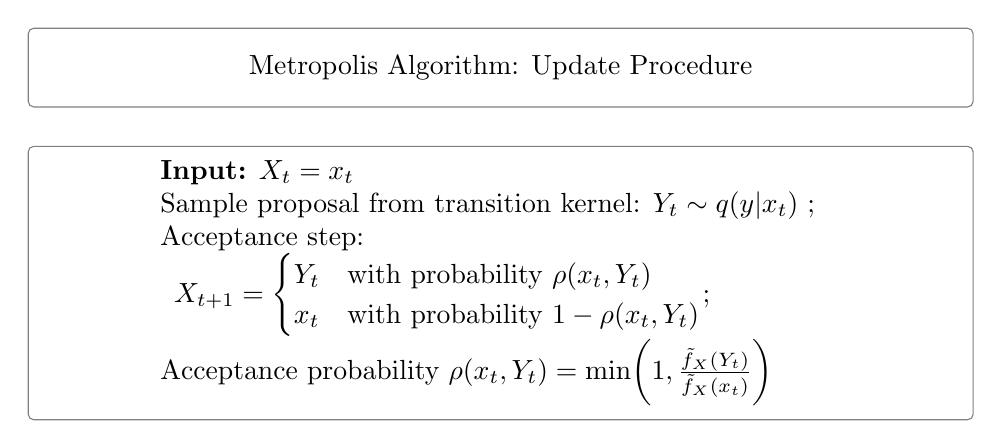
\begin{tikzpicture}
    \node[formula] (title) {Metropolis Algorithm: Update Procedure};
    \node[formula, below=0.5cm of title] (code) {%
            \begin{varwidth}{0.8\linewidth}
                \begin{algorithm}[H]
                    \KwIn{$X_t = x_t$}
                    Sample proposal from transition kernel: $Y_t \sim q(y | x_t)$ \;
                    Acceptance step: $X_{t+1} = \begin{cases}
                        Y_t & \text{with probability } \rho(x_t, Y_t)\\
                        x_t & \text{with probability } 1 - \rho(x_t, Y_t)
                    \end{cases}$\;
                    Acceptance probability $\rho(x_t, Y_t) = \min \biggl(1, \frac{\tilde{f}_X(Y_t)}{\tilde{f}_X(x_t)} \biggr) $
                \end{algorithm}%
        \end{varwidth}
%
            };
    % \node[formula, below=of title] (acceptance) { Acceptance probability: $\displaystyle \alpha = \min \biggl(1, \frac{\tilde{p}(\tilde{x})}{\tilde{p}(x_t)} \biggr)$, $\alpha \in (0, 1]$};
    % \node[formula, below=of acceptance] (uniform) {Reject sample if $U < \alpha$, where $U \sim \uniform (0, 1)$};
\end{tikzpicture}
\end{document}